% \newpage

\subsection{Scatter}
    The scatter operation is similar to broadcast, but instead of sending
    the entire message to all the other processes, the root process
    sends a different chunks of the message to each process. This is useful
    when the root process has a block of data that needs to be divided
    among all the other processes.
    The parameters for the tests are:
    \begin{itemize}
        \item iterations: 1000
        \item warmup: 100
        \item algorithms: basic linear, binomial
        \item message size: 1byte $\rightarrow$ 1 Mb
        \item number of processes: $2, 4, \dots, 48$
    \end{itemize}
    Like in the previous case we report the results considering the same
    three messages sizes. Again we expect to notice a significant increase
    in the latency when the MPI processes fill the socket and even more
    when they fill the node.
    \begin{figure}[H]
        \centering
        \resizebox{0.45\textwidth}{!}{
        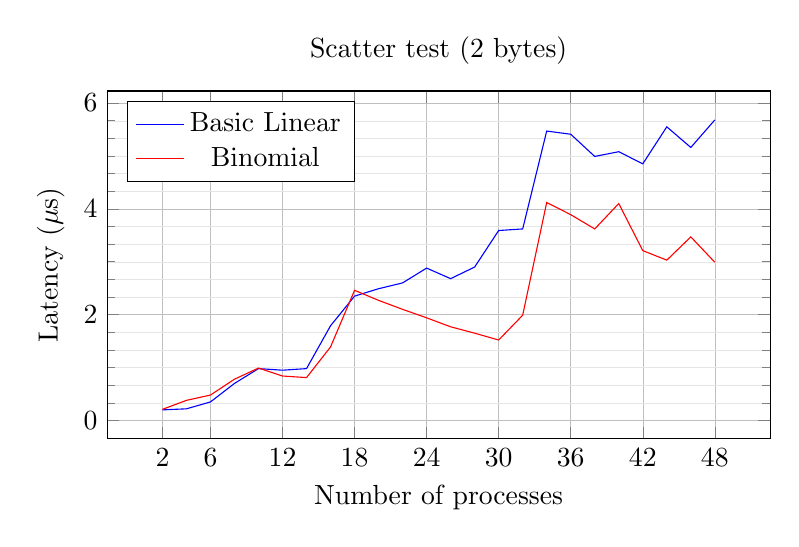
\begin{tikzpicture}
            \begin{axis}[
                title={Scatter test (2 bytes)},
                xlabel={Number of processes},
                ylabel={Latency ($\mu$s)},
                legend pos=north west,
                grid=both,
                grid style={line width=.1pt, draw=gray!20},
                major grid style={line width=.2pt,draw=gray!50},
                minor tick num=5,
                xtick={2, 6, 12, 18, 24, 30, 36, 42, 48},
                % xmode=log,
                % log basis x={2},
                % ymin=0,
                % xmin=0.5,
                % xmax=11.5,
                % xmax=100,
                % ytick={0, 50, 100, 150, 200, 250, 300, 350, 400},
                width=10cm,
                height=6cm,
                % cycle list name=color list,
            ]
            
            % x = [ 2  4  6  8 10 12 14 16 18 20 22 24 26 28 30 32 34 36 38 40 42 44 46 48]
            % basic-linear = [0.2  0.22 0.35 0.7  0.98 0.95 0.98 1.79 2.35 2.49 2.6  2.88 2.68 2.9 3.59 3.62 5.47 5.41 4.99 5.08 4.85 5.55 5.16 5.68]
            % binomial = [0.21 0.38 0.48 0.78 0.99 0.84 0.81 1.39 2.46 2.27 2.1  1.94 1.77 1.65 1.52 1.99 4.12 3.89 3.62 4.1  3.21 3.03 3.47 2.99]

            % Blue line: basic-linear
            \addplot[
                color=blue,
                mark=none,
                ]
                coordinates {
                (2, 0.2)
                (4, 0.22)
                (6, 0.35)
                (8, 0.7)
                (10, 0.98)
                (12, 0.95)
                (14, 0.98)
                (16, 1.79)
                (18, 2.35)
                (20, 2.49)
                (22, 2.6)
                (24, 2.88)
                (26, 2.68)
                (28, 2.9)
                (30, 3.59)
                (32, 3.62)
                (34, 5.47)
                (36, 5.41)
                (38, 4.99)
                (40, 5.08)
                (42, 4.85)
                (44, 5.55)
                (46, 5.16)
                (48, 5.68)
                };
                \addlegendentry{Basic Linear}

            % Red line: binomial
            \addplot[
                color=red,
                mark=none,
                ]
                coordinates {
                (2, 0.21)
                (4, 0.38)
                (6, 0.48)
                (8, 0.78)
                (10, 0.99)
                (12, 0.84)
                (14, 0.81)
                (16, 1.39)
                (18, 2.46)
                (20, 2.27)
                (22, 2.1)
                (24, 1.94)
                (26, 1.77)
                (28, 1.65)
                (30, 1.52)
                (32, 1.99)
                (34, 4.12)
                (36, 3.89)
                (38, 3.62)
                (40, 4.1)
                (42, 3.21)
                (44, 3.03)
                (46, 3.47)
                (48, 2.99)
                };
                \addlegendentry{Binomial}

            \end{axis}
        \end{tikzpicture}
        }
    \end{figure}
    For a small message size of 2 bytes, the binomial tree algorithm
    outperforms the basic linear one. 


    \begin{figure}[H]
        \centering
        \resizebox{0.45\textwidth}{!}{
        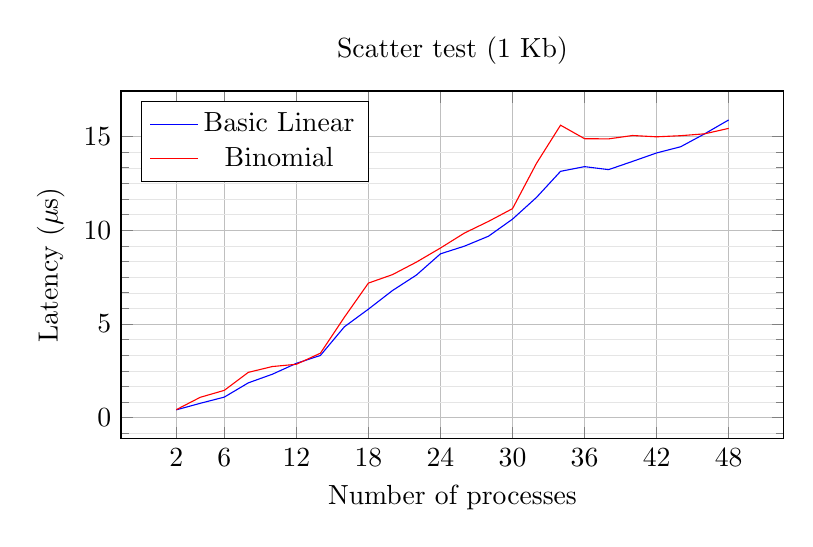
\begin{tikzpicture}
            \begin{axis}[
                title={Scatter test (1 Kb)},
                xlabel={Number of processes},
                ylabel={Latency ($\mu$s)},
                legend pos=north west,
                grid=both,
                grid style={line width=.1pt, draw=gray!20},
                major grid style={line width=.2pt,draw=gray!50},
                minor tick num=5,
                xtick={2, 6, 12, 18, 24, 30, 36, 42, 48},
                % xmode=log,
                % log basis x={2},
                % ymin=0,
                % xmin=0.5,
                % xmax=11.5,
                % xmax=100,
                % ytick={0, 50, 100, 150, 200, 250, 300, 350, 400},
                width=10cm,
                height=6cm,
                % cycle list name=color list,
            ]
            
            % x = [ 2  4  6  8 10 12 14 16 18 20 22 24 26 28 30 32 34 36 38 40 42 44 46 48]
            % basic-linear = [ 0.42  0.77  1.1   1.86  2.32  2.9   3.32  4.85  5.79  6.78  7.61  8.74  9.15  9.68 10.59 11.75 13.14 13.39 13.23 13.67 14.12 14.45 15.14 15.88]
            % binomial = [ 0.43  1.09  1.46  2.42  2.73  2.85  3.44  5.36  7.18  7.63  8.3   9.05  9.85 10.47 11.15 13.57 15.6  14.88 14.87 15.05 14.98 15.04 15.14 15.43]

            % Blue line: basic-linear
            \addplot[
                color=blue,
                mark=none,
                ]
                coordinates {
                (2, 0.42)
                (4, 0.77)
                (6, 1.1)
                (8, 1.86)
                (10, 2.32)
                (12, 2.9)
                (14, 3.32)
                (16, 4.85)
                (18, 5.79)
                (20, 6.78)
                (22, 7.61)
                (24, 8.74)
                (26, 9.15)
                (28, 9.68)
                (30, 10.59)
                (32, 11.75)
                (34, 13.14)
                (36, 13.39)
                (38, 13.23)
                (40, 13.67)
                (42, 14.12)
                (44, 14.45)
                (46, 15.14)
                (48, 15.88)
                };
                \addlegendentry{Basic Linear}

            % Red line: binomial
            \addplot[
                color=red,
                mark=none,
                ]
                coordinates {
                (2, 0.43)
                (4, 1.09)
                (6, 1.46)
                (8, 2.42)
                (10, 2.73)
                (12, 2.85)
                (14, 3.44)
                (16, 5.36)
                (18, 7.18)
                (20, 7.63)
                (22, 8.3)
                (24, 9.05)
                (26, 9.85)
                (28, 10.47)
                (30, 11.15)
                (32, 13.57)
                (34, 15.6)
                (36, 14.88)
                (38, 14.87)
                (40, 15.05)
                (42, 14.98)
                (44, 15.04)
                (46, 15.14)
                (48, 15.43)
                };
                \addlegendentry{Binomial}

            \end{axis}
        \end{tikzpicture}
        }
    \end{figure}
    \begin{figure}[H]
        \centering
        \resizebox{0.45\textwidth}{!}{
        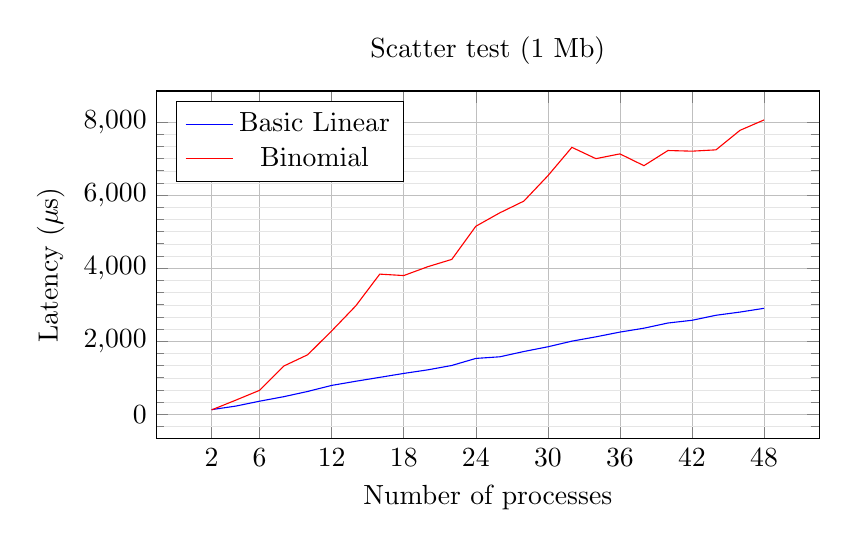
\begin{tikzpicture}
            \begin{axis}[
                title={Scatter test (1 Mb)},
                xlabel={Number of processes},
                ylabel={Latency ($\mu$s)},
                legend pos=north west,
                grid=both,
                grid style={line width=.1pt, draw=gray!20},
                major grid style={line width=.2pt,draw=gray!50},
                minor tick num=5,
                xtick={2, 6, 12, 18, 24, 30, 36, 42, 48},
                % xmode=log,
                % log basis x={2},
                % ymin=0,
                % xmin=0.5,
                % xmax=11.5,
                % xmax=100,
                % ytick={0, 50, 100, 150, 200, 250, 300, 350, 400},
                width=10cm,
                height=6cm,
                % cycle list name=color list,
            ]
            
            % x = [ 2  4  6  8 10 12 14 16 18 20 22 24 26 28 30 32 34 36 38 40 42 44 46 48]
            % basic-linear = [ 126.    222.22  357.39  479.9   623.76  789.07  902.46 1009.64 1117.33 1214.94 1334.99 1527.82 1572.21 1717.11 1846.12 2000.56 2118.62 2248.57 2355.12 2497.02 2571.44 2709.02 2796.63 2899.43]
            % binomial = [ 119.    383.83  655.32 1317.49 1628.77 2281.66 2964.79 3835.27 3795.96 4038.36 4238.62 5145.24 5513.75 5834.19 6527.81 7305.75 6995.97 7126.84 6804.27 7219.02 7201.17 7237.19 7771.69 8055.83]

            % Blue line: basic-linear
            \addplot[
                color=blue,
                mark=none,
                ]
                coordinates {
                (2, 126)
                (4, 222.22)
                (6, 357.39)
                (8, 479.9)
                (10, 623.76)
                (12, 789.07)
                (14, 902.46)
                (16, 1009.64)
                (18, 1117.33)
                (20, 1214.94)
                (22, 1334.99)
                (24, 1527.82)
                (26, 1572.21)
                (28, 1717.11)
                (30, 1846.12)
                (32, 2000.56)
                (34, 2118.62)
                (36, 2248.57)
                (38, 2355.12)
                (40, 2497.02)
                (42, 2571.44)
                (44, 2709.02)
                (46, 2796.63)
                (48, 2899.43)
                };
                \addlegendentry{Basic Linear}

            % Red line: binomial
            \addplot[
                color=red,
                mark=none,
                ]
                coordinates {
                (2, 119)
                (4, 383.83)
                (6, 655.32)
                (8, 1317.49)
                (10, 1628.77)
                (12, 2281.66)
                (14, 2964.79)
                (16, 3835.27)
                (18, 3795.96)
                (20, 4038.36)
                (22, 4238.62)
                (24, 5145.24)
                (26, 5513.75)
                (28, 5834.19)
                (30, 6527.81)
                (32, 7305.75)
                (34, 6995.97)
                (36, 7126.84)
                (38, 6804.27)
                (40, 7219.02)
                (42, 7201.17)
                (44, 7237.19)
                (46, 7771.69)
                (48, 8055.83)
                };
                \addlegendentry{Binomial}


            \end{axis}
        \end{tikzpicture}
        }
    \end{figure}


